\section{Quantiles Sketch}
\label{sec:quantiles}

\subsection{Overview}

Given a stream $A$ of items from an ordered domain, for every
$0< \phi < 1$, $\phi - quantile$ of $A$ is an item with rank 
$\lfloor \phi \cdot |A| \rfloor$, where the rank of item $i$ is the
number of elements in $A$ smaller than $i$.
An $\epsilon -approximate ~\phi - quantile$ is an element
with rank between $ (\phi - \epsilon) |A|$ and $ (\phi +
\epsilon) |A|$.
For every stream $A$, error $\epsilon$ and probability $\delta$,
a quantiles sketch algorithm produces a summary of $A$, which
supports $\epsilon -approximate ~\phi - quantile$ queries for
every $0< \phi < 1$ with probability at least $1 - \delta$.

As in the $\Theta$ sketch presented in the previous section, there
is a trade-off between summaries space cost and query accuracy,
which has been widely studied in the past.
In this work we build on top of an algorithm presented
in~\cite{}, which storage cost grows logarithmically with the
input stream size.
Given a stream $A$, the storage cost of the algorithm is
$k*2^{log(\lfloor |A|/k \rfloor)}$, where $k = O((1/\epsilon)
\sqrt{log(1/\epsilon \delta)}$.
The main idea of the algorithm is a simple technique to
\emph{merge} two sets, $S_1$ and $S_2$ of $k$ items each, to a
single set $S$ of $k$ items:
First, set $S = S_1 \cup S_2$, and sort $S$. 
Then, with equal probability, retain either the even or the odd
items in the sorted order. 
This process is called \emph{zip}.


The algorithm maintains $\lfloor log(|A|/k) \rfloor$ weighted
levels, where each level is an array of size $k$ that either contains $k$ ordered
items or invalid (also called empty).
The weight of level $i$ is $2^{i-1}$.
In addition to the levels arrays, the algorithm uses a
\emph{bitPattern} variable that indicates what levels are valid,
and a \emph{baseBuffer} of size $2k$, which is filled with items
from the stream.
Every time the baseBuffer is full, it is prop (in place) to
the levels arrays in the following way:
First we use the bitPattern to find the first invalid level in
the levels array. 
We call this level the \emph{target} level, and at the end of
the propagation this level will become valid, while all the the
level beneath it will be invalid.
Next, we sort and zip the base buffer (with equal probability,
pick either the even or the odd items in the sorted order) into
the target level.
And then we repeat the following process from level $i=1$ to the
last level that precedes the target level:
Mergesort level $i$ with what is currently stored in the target
level into the base buffer, and then zip the base buffer into the
target level.
Finally, update the bitPattern to indicate that all the target
level is now valid while all the level beneath are not.

Note that the weight of level $i+1$ is twice the wight of level
$i$ because it was zipped one more time, and thus it
``represents'' twice of the number of items ``represented'' in
level $i$.
This is important for quantiles accuracy.
In order to get a quantile we first have to build an
\emph{auxiliry} objects that contains two arrays:
(1) Sorted array of items, \emph{Iarr}, which 
contains all the items from all the valid levels, and (2) an
array of weights, called \emph{Warr}, that maps every item in
Iarr to its weight.
Then, to get the $~\phi - quantile$ of a stream $A$
we need to find the first index $ind$ in $Warr$ such that the
sum of all weights in $Warr$ till index $ind$ is $\lfloor \phi |A|
\rfloor$, and return $Iarr[ind]$.
Figure~\ref{fig:quantilesMerge} illustrates the algorithm.
Since it is not the focus of our paper we omit the error analysis
of the algorithm, and refer the interested reader to~\cite{} for
the proof and more details.

\begin{figure}[H]
    \centering
    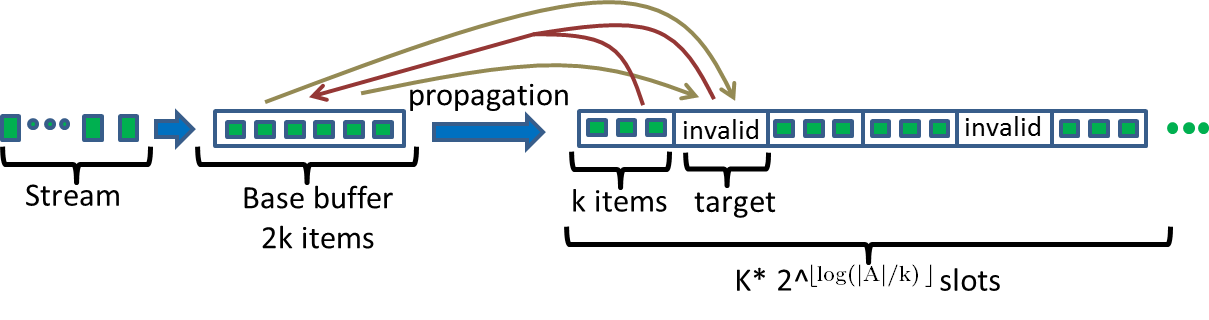
\includegraphics[width=5in]{images/quantilesPropogation.png}
    \caption{Quantile sketch. Propagation of the base buffer
    into the levels array.}
    \label{fig:quantilesMerge}
\end{figure}

The sequential implementation for $\Theta$ sketch is given in Algorithm~\ref{alg:sequential-quantiles}

\begin{algorithm}[htb]
\small
%\begin{multicols}{2}
\begin{algorithmic}[1]

	%\State {\bf Sketch variables:}
	\Vars
	\State \emph{sampleSet}, init $[ ]$ \Comment saved samples
	\State \emph{baseBuffer}, init $[ ]$ \Comment array of size 2K
	\State \emph{bitPattern}, init 0 \Comment bit array of valid levels in \emph{sampleSet}
	\EndFor

	\Statex
	\Procedure{query}{$\phi$}
	\State $tuples \leftarrow [ ]$
	\State $N \leftarrow 0$
	\ForAll{\emph{sample} in \emph{baseBuffer}}
		\State append $\langle$\emph{sample.val},\emph{$1$}$\rangle$ to \emph{tuples}
		\State $N \leftarrow N + 1$
	\EndFor
	\ForAll{\emph{lvl} s.t. bit \emph{lvl} is 1 in \emph{bitPattern}}
		\ForAll{\emph{sample} in \emph{sampleSet[lvl]}}
			\State append $\langle$\emph{sample.val},\emph{$2^{lvl}$}$\rangle$ to \emph{tuples}
		\EndFor
		\State $N \leftarrow N + 2^{lvl}k$
	\EndFor
	\State sort $tuples$ by $val$
	\State $pos \leftarrow \min {\{\lfloor N \times \phi \rfloor, N-1\}}$
	\State $sum \leftarrow 0$
	\State $ind \leftarrow 0$
	\While{$sum \leq pos$}
		\State $sum \leftarrow sum + tuples[ind].weight$
		\State $ind \leftarrow ind + 1$
	\EndWhile
	\State \Return $tuples[ind-1].val$ 
	\EndProcedure

	\Statex
	\Procedure{update}{$\langle val$,$coin \rangle$}
	\State ordered insert $\langle val$,$coin \rangle$ into \emph{baseBuffer} by \emph{val}
	\If{num items in \emph{baseBuffer} = $2K$}
		\State $tmpK \leftarrow$ \Call{zip}{baseBuffer}
		\State \Call {propogate}{\emph{tmpK, 0}}
		\State \emph{baseBuffer} $\leftarrow [ ]$ 
	\EndIf
	\EndProcedure

	\Statex
	\Procedure{union}{$S$}
	\For{\emph{lvl} s.t. bit \emph{lvl} is 1 in \emph{S.bitPattern}}
		\State $tmpK \leftarrow S.samepleSet[lvl]$
		\Call{propogate}{\emph{tmpK, lvl}}
	\EndFor
	\EndProcedure

	\Statex
	\Procedure{zip}{\emph{array}}
		\State $startIndex \leftarrow array[0].coin \oplus \dots \oplus array[2K].coin$
		\State $zipped \leftarrow [ ]$
		\State $index \leftarrow startIndex$
		\While{\emph{index} $<$ \emph{2K}}
			\State append \emph{array[index]} to \emph{zipped}
			\State $index \leftarrow index + 2$
		\EndWhile
		\State \Return{zipped}
	\EndProcedure

	\Statex
	\Procedure{propagate}{\emph{tmpK, startLvl}}
		\State \emph{target} $\leftarrow$ leftmost zero bit in \emph{bitPattern} after bit $startLvl$
		\State \emph{bitPatternMask} $\leftarrow$ 0
		\For{$lvl \in \{startLvl,\dots,target-1\}$}
				\State \emph{tmp2K} $\leftarrow$ mergeSort of \emph{tmpK} with \emph{sampleSet[lvl]}
				\State \emph{tmpK} $\leftarrow$ \Call{zip}{tmp2K}
				\State set bit \emph{lvl} in \emph{bitPatternMask} to 1
		\EndFor
		\State \emph{bitPatternMask[target]} $\leftarrow$ 1
		\If{\emph{target}=\emph{maxLevel}}
			\State wait until $\emph{bitPattern[maxLevel]}$ = 0
		\EndIf
		\State \emph{sampleSet[target]} $\leftarrow$ \emph{tmpK}
		\State {\tt atomic} \emph{bitPattern} $\leftarrow$ \emph{bitPattern} $\oplus$ \emph{bitPatternMask}
	\EndProcedure

\end{algorithmic}
%\end{multicols}
\caption{Sequential Quantiles sketch algorithm.}
\label{alg:sequential-quantiles}
\end{algorithm}

\subsection{Composable algorithm}

Recall that in order to read (getQuantiles), readers build an
auxiliary object based on the levels array and the bitPattern
that describes it.
Therefore, in order to be able to read concurrently with
background propagation, a reader must obtain a snapshot of the
levels array.
We solve it with the double successful collect technique.
First, we define the \emph{bitPattern} to be atomic in order to make sure
that a propagation is visible to all readers after the
\emph{bitPattern} is updated.

Recall that during the propagation process, the background
thread may read many levels, but writes only to the target level,
which is invalid at this point.
Therefore, a reader can be sure that the valid levels it reads
between the two identical reads of the bitPattern are consistent
even though the background thread concurrently
propagating.

In addition, note that a reader do not have to read all the valid
levels each time it fails to obtain a successful double collect.
Since a valid level may become invalid and then valid again
(with different items) only after a higher invalid level become
valid, if two sequential reads of the \emph{bitPattern} has a
common suffix, the reader must read only the valid levels in
the different prefix of the later \emph{bitPattern} read. 
It is guaranteed that the valid levels in the suffix are
unchanged.

Note that obviously the reads are not wait-free since the
\emph{bitPattern} can potently be changed faster than the readers ability
to read.
However, note that the propagation time (and thus
the time between \emph{bitPattern} changes) is longer when the target
level is higher, and once in a while the background thread must
propagate to high levels.
So, eventually the propagation will be long enough for
all the reader to obtain a snapshot of the levels array. 
However practically, we see that the readers are able to do it
much faster, and the snapshot time is negligible to the time to
build the auxiliary object.

A Quantile sketch \emph{copy} needs to copy only the arrays for which the bit in \emph{bitPattern}
is set, which symbolises a valid level. The method \emph{isFresh} needs only check equality
between the two \emph{bitPattern} values, as if they are equal no change was done to the valid levels.
The method \emph{shouldAdd} always returns true, as the sketch needs to add every element. This
means that \emph{calcHint} needs to return any value greater than 0, so it returns 1.
The composable implementation for Quantiles sketch is given in Algorithm~\ref{alg:composable-quantiles}.
Figure~\ref{fig:concurrentQuantiles} illustrates the concurrent
quantiles sketch architecture.

\begin{figure}[H]
    \centering
    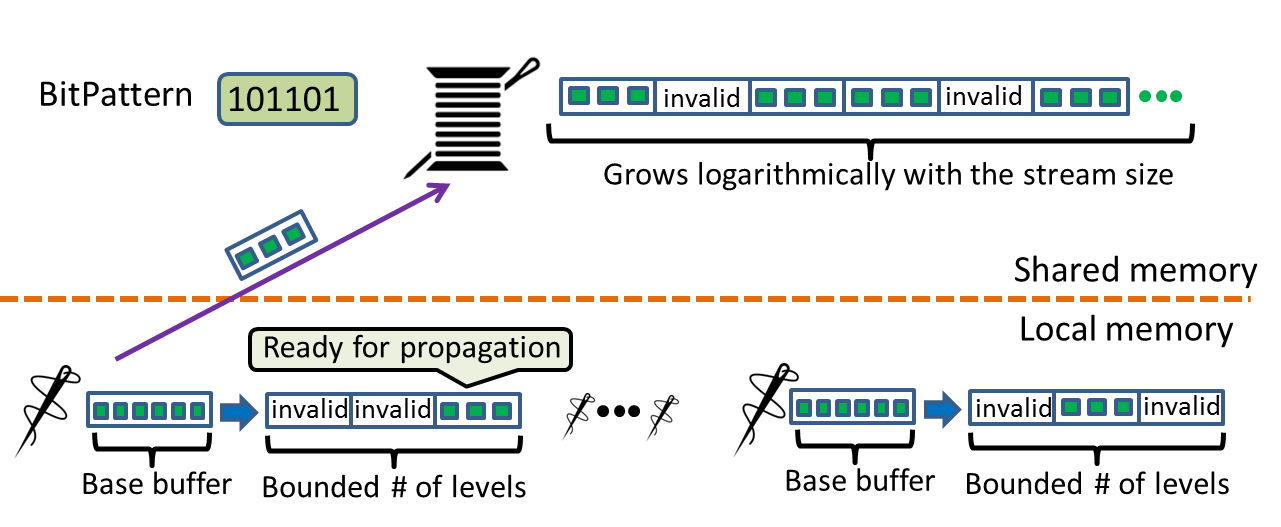
\includegraphics[width=5in]{images/concurrentQuantiles.png}
    \caption{Composable Quantile sketch.}
    \label{fig:concurrentQuantiles}
\end{figure}

\iffalse
Obviously protecting the sketch with a read/write lock yields
terrible performance. 
Not only that the fence decreases the throughput by a factor of 3
in update only scenario, but also since getting the quantiles
(reading) requires expensive computation, if we do it under lock
in mixed workload the throughput crashes.

Unfortunately, avoiding the lock is not an easy task. 
Since the propagation process (from the base buffer to levels
array), which requires most of the work in the algorithm, is
inherently very sequential, it cannot be done in parallel.
However, we can decrease the propagation rate without changing
the value of $k$. 
In other words, instead of propagating every $2k$ items we can
do it every $2^{i}k$, where $i \geq 0$ is a parameter that
impact accuracy (as described below).
This way we amortized the propagation cost and thus increase
throughput.

Our approach here is again to exploit locality and minimize
synchronization.
As in the concurrent $\Theta$ sketch, the idea is to have one
background thread and many worker threads.
Every worker thread maintains a local sketch with bounded number
of levels, and every time the local sketch fulfils, it passes
its last level to the background thread to propagate it to the
shared sketch.
In order to reduce the number of prop items to $k$, we
propagate when the last level of the local sketch is the only
valid level.
For a sketch with $i$ local levels, it happens every $2^ik$
items from the stream.
%Note also that if a thread have $i$ local levels, it passes $k$
%items to the background thread every $2^ik$ items from the
% stream.
The optimal number of local levels depends on the number of
concurrent worker threads.
Since we have only one background thread, the propagation
throughput is constant.
Meaning that when we have more worker threads, each thread gets
less help from the background thread, and thus
we need to make sure each thread needs the background thread
less often.
Therefore, for perfect scalability we increase the number of
local levels with the number of worker threads.

After asking the background thread to propagate its last level,
a worker thread starts filling its local sketch again, hoping the
propagation process will complete faster.
The synchronization between the
background thread and a worker thread $t_i$ is done over a
single atomic bit array $bitPattern$.

To propagate level $i$ from a local sketch to the shared sketch,
the background thread uses the mechanism described in the
sequential quantiles sketch overview above with the following
change:
Instead of starting from zipping the base buffer
into the target level, it starts from level $i$.
If level $i$ in the shared sketch is valid, the background
thread merges it (via merge sort) with the local level $i$ into
the base buffer, and continue the propagation to the next level
as before.
Otherwise, it simple copy the local level $i$ to the shared level
$i$.
The target buffer in this case is the first invalid level that is
not smaller than $i$.
Figure~\ref{cocurrentQuntiles} illustrates the concurrent
quantiles sketch architecture.

Recall that in order to read (getQuantiles), readers build an
auxiliary object based on the levels array and the bitPattern
that describes it.
Therefore, in order to be able to read concurrently with
background propagation, a reader must obtain a snapshot of the
levels array.
We solve it with the double successful collect technique.
First, we define the bitPattern to be atomic in order to make sure
that a propagation is visible to all readers after the
bitPattern is updated.
Second, a reader repeatedly tries to obtain a consistent query from
the globalS: it reads the bitPattern, then activates query,
and then reads the bitPattern again.
If the bit pattern did not change between the two reads, the
reader has a consistent view.
Otherwise, it tries again.

Recall that during the propagation process, the background
thread may read many levels, but writes only to the target level,
which is invalid at this point.
Therefore, a reader can be sure that the valid levels it reads
between the two identical reads of the bitPattern are consistent
even though the background thread concurrently
propagating.
%In addition, note that a reader do not have to read all the valid
%levels each time it fails to obtain a successful double collect.
%Since a valid level may become invalid and then valid again
%(with different items) only after a higher invalid level become
%valid, if two sequential reads of the bitPattern has a
%common suffix, the reader must read only the valid levels in
%the different prefix of the later bitPattern read. 
%It is guaranteed that the valid levels in the suffix are
%unchanged.

Note that obviously the reads are not wait-free since the
bitPattern can potently be changed faster than the readers ability
to read.
However, note that the propagation time (and thus
the time between bitPattern changes) is longer when the target
level is higher, and once in a while the background thread must
propagate to high levels.
So, eventually the propagation will be long enough for
all the reader to obtain a snapshot of the levels array. 
However practically, we see that the readers are able to do it
much faster, and the snapshot time is negligible to the time to
build the auxiliary object.
\fi

\begin{algorithm}[tb]
	\small
	\begin{multicols}{2}
	\begin{algorithmic}[1]
	
		\Vars
		\State \emph{sampleSet}, init $[ ]$ \Comment saved samples
		\State \emph{baseBuffer}, init $[ ]$ \Comment array of size 2K
		\State \emph{bitPattern}, init 0 \Comment bit array of valid levels in \emph{sampleSet}
		\State \emph{maxLevel}, init $\infty$ \Comment max level of \emph{sampleSet}
		\EndFor
	
		\Statex
		\Procedure{fresh}{S}
			\State return $bitPattern == S.bitPattern$
		\EndProcedure
	
		\Statex
		\Procedure{copy}{$T$}
			\State $currentBitPattern \leftarrow bitPattern$
			\State $diff \leftarrow currentBitPattern \oplus T.bitPattern$
			\State $maxDiff \leftarrow $ rightmost $1$ bit in $diff$
			\ForAll{$lvl \in \Collection{1,\dots,maxDiff}$}
			\If{bit $lvl$ in $bitPattern$ is $1$}
				$T.sampleSet[lvl] \rightarrow sampleSet[lvl]$
			\EndIf
			\EndFor
			\State $T.bitPattern \leftarrow currentBitPattern$
			\Return $T$
		\EndProcedure
	
		\Statex
		\Procedure{calchint}{}
			\Return $1$
		\EndProcedure
	
		\Statex
		\Procedure{shouldAdd}{P, arg}
			\Return $true$
		\EndProcedure
	
	\end{algorithmic}
	\end{multicols}
	\caption{Composable quantiles sketch.}
	\label{alg:composable-quantiles}
	\end{algorithm}


\subsection{Analysis}
In order to capture the randmoness of the zip operation, we will model the values provided in the stream
as arriving in tuple form $\langle$\emph{val},\emph{C}$\rangle$, where $C\in\{0,1\}$, the that values of
\emph{C} provided externally. The zip operation performs $C_1 \oplus C_2 \oplus \dots \oplus C_{2K}$, and if
the answer is 0 then the operation chooses the even places in the set, if 1 then the odd places. As in $\Theta$,
the correctness is derived from the generic algorithm, we need only prove that the additional methods adhere 
to the requirements set upon them.

The $copy$ method copies the entire sketch. It is easy to see that if no updates are happening concurrently
to a $copy$, the returned sketch is a copy. In this case the sketch's are equal, therefore the $bitPattern$s
are equal, and then $fresh$ returns true as long as no updates have been done to the original sketch.

Also, the method $shouldAdd$ returns true always, therefore adheres to the requirement set upon it
immediately.